% Tension Mining: A Structured Methodology for Cross-Domain Invariant Discovery
% arXiv submission — cs.MA primary, cross-list cs.CY, cs.SI
%
% Compile: pdflatex -> bibtex -> pdflatex -> pdflatex

\documentclass[11pt,a4paper]{article}

% ---- Packages ----
\usepackage[utf8]{inputenc}
\usepackage[T1]{fontenc}
\usepackage{microtype}
\usepackage{geometry}
\geometry{margin=1in}
\usepackage{setspace}
\singlespacing

\usepackage{graphicx}
\usepackage{amsmath,amssymb}
\usepackage{hyperref}
\hypersetup{
  colorlinks=true,
  linkcolor=blue,
  citecolor=blue,
  urlcolor=blue
}
\usepackage{natbib}
\bibliographystyle{plainnat}
\usepackage{booktabs}
\usepackage{array}
\usepackage{caption}
\usepackage{subcaption}
\usepackage{tikz}
\usetikzlibrary{shapes.geometric, arrows, positioning, fit}

% ---- Commands ----
\newcommand{\methodname}{Tension Mining}
\newcommand{\pipeline}{Phenomenon Mining $\rightarrow$ Tension Mining $\rightarrow$ Invariant Mining $\rightarrow$ Mechanism Mining $\rightarrow$ System Synthesis $\rightarrow$ Algorithm Synthesis $\rightarrow$ Destruction}

% ---- Document ----
\begin{document}

\title{\textbf{\methodname}: A Structured Methodology for Cross-Domain Invariant Discovery in Complex Systems}

\author{Ceaser Zhao\\[4pt]
\small Independent Researcher\\
\small \texttt{https://github.com/zbbsdsb/Tension-Mining}}

\date{}

\maketitle

\begin{abstract}
Most innovation workflows in complex systems begin with algorithms, architectures, or implementations, bypassing a critical preliminary question: what persistent forces shape this system? We present \methodname, a structured 7-phase methodology for discovering cross-domain invariants---principles that remain valid across seemingly unrelated domains---by systematically mining the underlying tensions that define a system's behavior. The pipeline progresses from concrete observations (Phenomenon Mining) through tension identification, invariant extraction, mechanism study, system synthesis, and algorithm derivation, concluding with an adversarial Destruction Phase that stress-tests the resulting model. We demonstrate the methodology through case studies of PageRank (information retrieval) and Bitcoin (cryptocurrency), showing how both landmark systems emerged not from algorithmic optimization but from making hidden tensions visible. \methodname is designed as an AI-executable skill and is accompanied by an open-source reference implementation with 11 case studies across 7 domains, 19 cataloged tensions, and 12 validated invariants.
\end{abstract}

% ======================================================================
\section{Introduction}
\label{sec:introduction}
% ======================================================================

The history of influential complex systems reveals a recurring pattern. PageRank began not with a matrix equation but with a question about the nature of importance in networked information~\cite{page1999pagerank}. Bitcoin emerged not from a blockchain data structure but from a tension between decentralization and trust in digital transactions~\cite{nakamoto2008bitcoin}. The Transformer architecture did not originate from an attention mechanism but from questioning whether recurrence was necessary at all~\cite{vaswani2017attention}. Wikipedia was not conceived as a revision control system but as a response to the tension between open participation and content reliability~\cite{vygotsky1978mind}.

In each case, the breakthrough was not algorithmic --- it was conceptual. The inventors first made visible a hidden tension, and the algorithms followed naturally.

Despite this pattern, the dominant methodology for designing complex systems remains solution-first: identify a problem domain, design an algorithm, optimize. This approach works well for well-defined problems in ordered domains but frequently fails in complex domains where the fundamental tradeoffs are not yet understood~\cite{snowden2007leader}.

We propose \methodname, a structured methodology that inverts the traditional design sequence. Instead of starting from solutions, it starts from reality: collect phenomena from multiple domains, identify the persistent tensions underlying them, extract cross-domain invariants, study how reality resolves these tensions, and only then derive algorithms. The pipeline consists of seven phases, each with explicit gate conditions that prevent premature solution-jumping.

The methodology makes three contributions:

\begin{enumerate}
  \item \textbf{A formal pipeline} for moving from observations to invariants to algorithms, with anti-cheat mechanisms that resist the human tendency to skip to solutions.
  \item \textbf{A tension-centric ontology} that reframes system analysis around \emph{ineliminable tradeoffs} rather than features or requirements.
  \item \textbf{An open, executable implementation} published as a Markdown-based AI Skill, enabling researchers and practitioners to apply the methodology through existing AI tools.
\end{enumerate}

\methodname is not a replacement for existing methodologies but a complement. It is designed for the early, conceptual phase of system design --- the phase that occurs before problem framing is complete and before any algorithm has been selected. It is most valuable when the domain is poorly understood, when cross-domain analogies might yield insight, or when existing approaches have reached diminishing returns.

% ======================================================================
\section{Related Work}
\label{sec:related}
% ======================================================================

\methodname draws on and synthesizes multiple research traditions. We position it relative to four closely related methodologies.

\subsection{Design Thinking}
Design Thinking~\cite{schon1983reflective,cross2006designerly} emphasizes empathy, ideation, and rapid prototyping. It is fundamentally solution-oriented: the goal is to produce a prototype that addresses user needs. \methodname is understanding-oriented: the goal is to produce a tension map and invariant set before any solution is considered. The two are complementary. Design Thinking excels at ``how might we solve this?''; \methodname addresses ``what forces are shaping this system?''.

\subsection{Systems Dynamics}
Systems Dynamics~\cite{meadows2008thinking} models systems through causal loop diagrams, stocks, flows, and feedback loops. It is quantitative, precise, and domain-specific. \methodname operates at a higher level of abstraction, seeking \emph{cross-domain} invariants rather than domain-specific dynamics. A systems dynamics model predicts behavior within a known structure; \methodname seeks to discover the structure itself.

\subsection{Cynefin Framework}
The Cynefin framework~\cite{snowden2007leader} classifies problems into five domains (Clear, Complicated, Complex, Chaotic, Disorder) and prescribes different decision-making approaches for each. \methodname can be seen as a methodology specialized for the Complex domain of Cynefin, where cause-and-effect relationships are not known in advance and must be discovered through pattern recognition.

\subsection{First Principles Thinking}
First Principles reasoning decomposes a problem into its fundamental truths and rebuilds from there. \methodname shares this reductionist spirit but differs in its object of inquiry: First Principles asks ``what is this made of?''; \methodname asks ``what forces cannot be eliminated?''. The output of First Principles is a decomposed understanding; the output of \methodname is a set of invariants.

\subsection{Positioning}
No existing methodology provides a structured, phase-gated pipeline specifically designed for discovering cross-domain invariants from persistent tensions. \methodname fills this gap by combining elements of all four approaches into a single, executable framework with explicit anti-cheat mechanisms and quality rubrics.

% ======================================================================
\section{Methodology}
\label{sec:methodology}
% ======================================================================

\methodname consists of seven phases, executed in strict order. Each phase has a \emph{gate condition} that must be satisfied before proceeding. The pipeline is visualized in Figure~\ref{fig:pipeline}.

\begin{figure}[t]
\centering
\begin{tikzpicture}[
  node distance=0.8cm and 0.3cm,
  phase/.style={rectangle, rounded corners, draw=black!70, fill=black!5,
    minimum width=4.2cm, minimum height=0.7cm, align=center, font=\small\bfseries},
  arrow/.style={->, thick, black!60},
  sublabel/.style={font=\scriptsize, text=black!50, align=center}
]

% Row 1: Phase names
\node[phase] (P1) {Phenomenon Mining};
\node[phase, right=of P1] (P2) {Tension Mining};
\node[phase, right=of P2] (P3) {Invariant Mining};
\node[phase, right=of P3] (P4) {Mechanism Mining};
\node[phase, right=of P4] (P5) {System Synthesis};
\node[phase, right=of P5] (P6) {Algorithm Synthesis};
\node[phase, right=of P6, fill=black!10, draw=black] (P7) {Destruction};

% Arrows between phases
\foreach \i/\j in {P1/P2, P2/P3, P3/P4, P4/P5, P5/P6, P6/P7} {
  \draw[arrow] (\i) -- (\j);
}

% Row 2: Gate conditions
\node[sublabel, below=0.15cm of P1] {Gate: $\ge$ 5 phenomena from $\ge$ 3 domains};
\node[sublabel, below=0.15cm of P2] {Gate: $\ge$ 3 ineliminable tensions};
\node[sublabel, below=0.15cm of P3] {Gate: $\ge$ 1 cross-domain invariant};
\node[sublabel, below=0.15cm of P4] {Gate: 1 mechanism per tension};
\node[sublabel, below=0.15cm of P5] {Gate: Coherent model with failure modes};
\node[sublabel, below=0.15cm of P6] {Gate: Algorithm derived from mechanism};
\node[sublabel, below=0.15cm of P7] {Gate: Assumptions falsified or narrowed};

% Row 3: Core questions
\node[sublabel, below=0.85cm of P1, font=\tiny\itshape] {\emph{``What already exists?''}};
\node[sublabel, below=0.85cm of P2, font=\tiny\itshape] {\emph{``What tradeoff persists?''}};
\node[sublabel, below=0.85cm of P3, font=\tiny\itshape] {\emph{``What repeats across domains?''}};
\node[sublabel, below=0.85cm of P4, font=\tiny\itshape] {\emph{``How does reality resolve it?''}};
\node[sublabel, below=0.85cm of P5, font=\tiny\itshape] {\emph{``What is the minimal model?''}};
\node[sublabel, below=0.85cm of P6, font=\tiny\itshape] {\emph{``What algorithm emerges?''}};
\node[sublabel, below=0.85cm of P7, font=\tiny\itshape] {\emph{``What breaks?''}};

\end{tikzpicture}
\caption{The 7-phase \methodname pipeline. Each phase has a gate condition that enforces completeness before progression. The Destruction Phase (Phase 7) is an adversarial self-evaluation that explicitly tests the model's robustness.}
\label{fig:pipeline}
\end{figure}

\subsection{Phase 1: Phenomenon Mining}

The practitioner collects 5--10 real-world examples of the target system's behavior from at least 3 distinct domains. The goal is not to find examples that confirm a hypothesis but to build a diverse phenomenon library. For a system like ``decentralized coordination'', phenomena might include ant colony foraging (biology), Wikipedia article editing (social), Bitcoin mining (cryptocurrency), and open-source software contribution (software engineering).

\textbf{Gate condition:} At least 5 phenomena from at least 3 domains. No two phenomena may come from the same domain.

\subsection{Phase 2: Tension Mining}

Each pair of forces that persistently pull the system in different directions is identified as a \emph{tension}. A tension is \emph{ineliminable}: it cannot be permanently resolved by any design choice, only managed. Examples include Local~$\leftrightarrow$~Global (information routing), Freedom~$\leftrightarrow$~Efficiency (collective action), and Autonomy~$\leftrightarrow$~Control (agent coordination).

\textbf{Gate condition:} At least 3 ineliminable tensions, each supported by phenomena from at least 2 domains.

\subsection{Phase 3: Invariant Mining}

From the identified tensions, the practitioner extracts invariants---principles that remain valid across domains. An invariant is not a tension but a statement about how tensions manifest. For example, ``Local Rules Create Global Order'' (I-LCG-001) states that local interactions between system components reliably produce global patterns without centralized control, an invariant observed across ant colonies, Wikipedia, and Bitcoin.

\textbf{Gate condition:} At least 1 cross-domain invariant, supported by phenomena from at least 3 domains.

\subsection{Phase 4: Mechanism Mining}

The practitioner studies how reality resolves or manages each identified tension. Mechanisms are existing processes --- biological, social, technological --- that handle tradeoffs without eliminating them. For the identity~$\leftrightarrow$~cooperation tension, mechanisms include reputation systems (social), kin selection (biological), and cryptographic signatures (technological).

\textbf{Gate condition:} At least one mechanism per tension. Each mechanism must be evidenced in a real system.

\subsection{Phase 5: System Synthesis}

Tensions, invariants, and mechanisms are combined into a coherent model. The model identifies which tensions are primary, which mechanisms are essential, and what failure modes exist. The synthesis should be the minimal model that explains the observed phenomena.

\textbf{Gate condition:} A coherent model that accounts for all phenomena. The failure modes must be explicitly stated.

\subsection{Phase 6: Algorithm Synthesis}

Only now does the practitioner design algorithms. Algorithms must emerge fluidly from the mechanisms identified in Phase 4, not be imported from unrelated domains. If an algorithm cannot be directly derived from a mechanism, the mechanism analysis is incomplete.

\textbf{Gate condition:} Each algorithm must be traceable to a mechanism from Phase 4. Algorithms with no mechanistic basis are excluded.

\subsection{Phase 7: Destruction}

The practitioner explicitly attempts to falsify the resulting model. What assumptions would need to be false for the model to fail? What edge cases break it? What tensions were missed? This adversarial self-evaluation is the most critical phase, as it guards against confirmation bias that accumulates through Phases 1--6.

\textbf{Gate condition:} At least 3 falsification attempts. At least 1 assumption must be either falsified or meaningfully refined.

\subsection{Anti-Cheat Mechanisms}

The methodology includes two mechanisms to resist the human tendency to skip phases:

\begin{enumerate}
  \item \textbf{Common Rationalizations Table:} Documented phrases that indicate phase-skipping, such as ``I already know the tensions, let's skip to the algorithm'' (rationalization: False urgency) or ``Let's do a quick Phase 1 and spend time on the algorithm'' (rationalization: Premature optimization).
  \item \textbf{Quality Rubric:} A 5-dimension scoring system (Depth, Breadth, Rigor, Novelty, Actionability) with a 15-point scale, appended to every \methodname output. Scores below 10 trigger an automatic restart from Phase 2.
\end{enumerate}

% ======================================================================
\section{Demonstration}
\label{sec:demonstration}
% ======================================================================

We demonstrate \methodname on two landmark systems from different domains: PageRank (information retrieval) and Bitcoin (cryptocurrency). These systems were selected because they are well-documented and their origins are not primarily algorithmic.

\subsection{Case Study 1: PageRank}

\textbf{Phase 1 -- Phenomena:} Academic citation networks (scientific publishing), web link structures (information science), social influence hierarchies (sociology), and city accessibility patterns (urban planning).

\textbf{Phase 2 -- Tensions:} Local~$\leftrightarrow$~Global (T-LOC-004): Importance is a global property, but computation must be local and iterative. Freedom~$\leftrightarrow$~Efficiency (T-FRE-006): Web authors freely link to any page, but efficient ranking requires well-structured graph navigation.

\textbf{Phase 3 -- Invariants:} Local Rules Create Global Order (I-LCG-001): The random surfer model converts local link-following behavior into global PageRank scores. Gradients Drive Movement (I-GDM-001): The PageRank algorithm computes a gradient of importance that flows through the link graph.

\textbf{Phase 4 -- Mechanisms:} Eigenvector centrality (mathematical), academic peer review (social), and citation chain propagation (informational) all address the local-global tension through iterative propagation.

\textbf{Phase 5 -- Synthesis:} The model describes the web as a citation graph where importance propagates along links, dampened by a decay factor that models the random surfer's likelihood of abandoning the current path.

\textbf{Phase 6 -- Algorithm:} The PageRank algorithm $PR(p) = (1-d)/N + d \sum_{q \in M(p)} PR(q)/L(q)$ emerges naturally from the mechanism. The damping factor $d$ directly encodes the tension between local exploration and global convergence.

\textbf{Phase 7 -- Destruction:} Vulnerabilities include link spam (artificial inflation of PageRank through link farms), the ``Google dance'' (instability during index updates), and the assumption that links are editorial endorsements (which fails for paid links).

\subsection{Case Study 2: Bitcoin}

\textbf{Phase 1 -- Phenomena:} Physical currency systems (economics), digital double-spending attempts (computer security), Byzantine Generals Problem (distributed systems), and commodity-based value storage (anthropology).

\textbf{Phase 2 -- Tensions:} Centralization~$\leftrightarrow$~Decentralization (T-CEN-011): Trusted intermediaries prevent double-spending but create centralized control. Competition~$\leftrightarrow$~Cooperation (T-COP-015): Miners compete for rewards but must cooperate on protocol rules.

\textbf{Phase 3 -- Invariants:} Identity Drives Cooperation (I-IDC-001): Bitcoin creates a pseudonymous identity system where cooperation (honest mining) is incentivized and defection (double-spending) is economically irrational. Tradeoffs Are Inescapable (I-TAE-001): Every optimization in blockchain design (block size, confirmation time, energy consumption) is a tradeoff between competing values.

\textbf{Phase 4 -- Mechanisms:} Proof-of-work (cryptographic), longest-chain rule (consensual), and economic game theory (incentive) collectively resolve the decentralization-trust tension by making dishonesty more expensive than honesty.

\textbf{Phase 5 -- Synthesis:} Bitcoin is a system where energy expenditure (proof-of-work) replaces trust, and economic incentives replace centralized enforcement. The model is stable only as long as the cost of attack exceeds the potential benefit.

\textbf{Phase 6 -- Algorithm:} The Nakamoto consensus algorithm combines proof-of-work, longest-chain selection, and block reward halving into a coherent protocol. Each component maps to a mechanism identified in Phase 4.

\textbf{Phase 7 -- Destruction:} Attack vectors include the 51\% attack (majority hash power), selfish mining (withholding blocks), and the governance tension (protocol changes require community consensus, which is slow and contentious).

% ======================================================================
\section{Discussion}
\label{sec:discussion}
% ======================================================================

\subsection{When the Methodology Works}

\methodname is most effective when the problem domain is complex (in the Cynefin sense), when cross-domain analogies are likely to yield insight, and when the designer is willing to defer algorithmic thinking until the system's tensions are understood. The methodology is well-suited to multi-agent systems, social computing platforms, cryptographic protocol design, and any domain where human and technical components interact non-trivially.

\subsection{Limitations}

The methodology has three important limitations. First, it produces qualitative insights, not quantitative predictions. It identifies \emph{what} forces shape a system but does not predict \emph{how much} each force matters. Second, the quality of output depends on the breadth of the phenomenon library in Phase 1. A narrow phenomenon set produces narrow invariants. Third, the methodology requires significant domain expertise to identify meaningful tensions; novice practitioners may produce trivial or overly general results.

\subsection{Open Implementation}

\methodname is published as an open-source Markdown-based AI Skill at \url{https://github.com/zbbsdsb/Tension-Mining}. The repository includes a complete Skill specification (\texttt{SKILL.md}), detailed phase instructions (\texttt{references/execution-protocol.md}), a tension atlas of 19 cataloged tensions (\texttt{references/tension-atlas.md}), an invariant atlas of 12 invariants (\texttt{references/invariant-atlas.md}), 11 full case studies (\texttt{examples/}), 9 domain templates (\texttt{templates/}), an automated validation script (\texttt{scripts/validate-atlas.py}), and a quality rubric (\texttt{references/quality-rubric.md})~\cite{knowls_repo}.

The Skill can be loaded into any AI tool that supports Markdown-based skill files (Claude Code, TRAE, Cursor, Windsurf). Automatic trigger keywords activate the methodology when a user describes a complex system design problem.

% ======================================================================
\section{Conclusion}
\label{sec:conclusion}
% ======================================================================

We have presented \methodname, a structured 7-phase methodology for discovering cross-domain invariants in complex systems by mining persistent tensions. The methodology inverts the conventional design sequence by starting with phenomena rather than solutions, and by requiring explicit gate conditions that prevent premature algorithmization. Two case studies (PageRank, Bitcoin) demonstrate how the pipeline recovers the conceptual breakthroughs that led to these influential systems.

The methodology is intentionally qualitative and open-ended. It is a lens, not a formula. Its value lies not in producing outputs that can be mechanically evaluated but in changing the sequence of questions a researcher asks when confronting a complex system. The most important question is not ``what algorithm should I build?'' but ``what tension am I not seeing?''.

% ======================================================================
\bibliography{tension-mining-arxiv}
% ======================================================================

\end{document}